\documentclass[10pt,a4paper]{article}

\usepackage[margin=0.85in]{geometry}
\usepackage{amsmath,amssymb}
\usepackage{tikz}
\usetikzlibrary{arrows.meta,positioning,fit,backgrounds,shapes.geometric,calc}
\usepackage{booktabs}
\usepackage{enumitem}
\usepackage{microtype}
\usepackage{xcolor}
\usepackage[hidelinks]{hyperref}
\usepackage[backend=biber,style=numeric,sorting=none,maxnames=3,minnames=1]{biblatex}
\addbibresource{references.bib}

\setlist{nosep,leftmargin=1.2em}

\title{\vspace{-3em}\textbf{LapEE: (Secure-ish) Laptop Execution Environments\\for Decentralized Compute on Untrusted Commodity Hardware}}

\author{%
  Claude Opus 4.7[1m]\\\small{Anthropic}
  \and
  Sam Williams\\\small{\texttt{sam@arweave.org}}
}

\date{April 2026}

\begin{document}
\maketitle
\vspace{-1.8em}

\begin{abstract}
\noindent
The prevailing view in decentralized compute is that meaningful hardware-backed
privacy and integrity require a Trusted Execution Environment of the kind
offered by Intel TDX, AMD SEV-SNP, or NVIDIA Confidential Compute. This view
is mistaken for the decentralized-compute threat model specifically, and
wastefully so. Four primitives shipped across commodity hardware over the last
five years --- TPM 2.0, UEFI Secure Boot with operator-enrolled trust anchors,
an IOMMU, and platform Total Memory Encryption (Intel TME, AMD SME/TSME) ---
together support a measured, attested, memory-encrypted, DMA-contained
single-purpose appliance for HyperBEAM~\cite{hyperbeam-repo}. The missing
feature of a classical hardware TEE --- multi-tenant isolation on a single
machine --- is not required for decentralized compute, which provides tenancy
\emph{between} machines. LapEE's running-workload TCB is the same order of
magnitude as a deployed confidential VM's; the installed base is roughly an
order of magnitude larger, at roughly one to two orders of magnitude lower
per-machine cost, often including hardware already in operators' possession
at zero cost. We contribute a threat model and trust-boundary analysis, an
architecture binding a per-boot ephemeral signing key to the fully-measured
stack via PCR extension and continued through AO-Core~\cite{ao-core}
hashpath, and a grounded hardware-availability survey.
\end{abstract}

\vspace{-0.5em}
\section{Introduction}
\vspace{-0.3em}

Decentralized compute wants hardware-rooted privacy and integrity on machines
owned by untrusted operators. The canonical answer --- Intel
TDX~\cite{intel-tdx}, AMD SEV-SNP~\cite{amd-snp}, NVIDIA Confidential Compute
--- is narrow: server silicon priced at \$10--50k, concentrated in cloud
providers. Attempts to extend onto consumer hardware, most visibly Apple
Silicon~\cite{naik-dginf}, run into the absence of any third-party-accessible
measurement register.

Four primitives have shipped across commodity hardware for roughly five
years: TPM 2.0~\cite{tcg-tpm2}, UEFI Secure Boot with operator-enrollable
trust anchors~\cite{uefi-spec}, an IOMMU (VT-d or AMD-Vi), and platform
memory encryption (Intel TME~\cite{intel-tme}, AMD SME/TSME~\cite{amd-sme}).
Composed, they produce an attested appliance: a machine that boots a signed,
locked-down, reproducibly-built image, encrypts all DRAM at the memory
controller, constrains peripheral DMA through the IOMMU, and proves what it
runs via a cryptographic chain rooted in the TPM vendor's signing key.

\paragraph{The trade.} Classical TEEs defend a single workload from other
privileged workloads \emph{on the same machine}. LapEE does not: exactly one
attested workload runs, nothing else. The network provides multi-tenancy
\emph{between} machines by distributing work, not within them by
partitioning. A different architectural choice, not a weaker one, and in a
permissionless network the correct one.

\paragraph{What LapEE is not.} (a) a classical hardware TEE; (b) a
multi-tenant single-machine execution environment; (c) a replacement for
cryptographic MPC or FHE; (d) a solution to traffic analysis or liveness.

\paragraph{Who has the hardware.} Every 2020$+$ business-class laptop
(Intel vPro, AMD Ryzen Pro), Xeon Scalable server since Ice Lake-SP, and
EPYC since Naples has the silicon. Business-class secondary-market refurbs
cost hundreds of dollars; many operators already own suitable hardware. The
laptop is our paradigm: its integrated battery is a de-facto UPS smoothing
brief power loss, directly useful for node liveness.

\paragraph{Contributions.} (1) A threat model and trust-boundary analysis.
(2) An architecture binding a per-boot ephemeral signing key to the full
measured stack via PCR extension, continued through AO-Core to produce a
single merkle chain from firmware measurement to signed result.
(3) An honest analysis of plain-TME/SME's confidentiality and replay
properties, with concrete mitigations. (4) A grounded availability survey.

\vspace{-0.3em}
\section{Positioning}
\label{sec:positioning}
\vspace{-0.3em}

A classical hardware TEE provides (a) a hardware-signed measurement of the
workload and (b) hardware-enforced isolation from other privileged code on
the same machine. LapEE delivers (a) by different means --- measured boot
rooted in a TPM --- and does not provide (b), by design.

\begin{table}[ht]
\centering
\footnotesize
\begin{tabular}{@{}l p{0.77\linewidth}@{}}
\toprule
\textbf{System} & \textbf{Running-workload TCB} \\
\midrule
SGX (historic) & CPU $+$ microcode $+$ SGX runtime $+$ enclave code. Small. Deprecated on consumer parts~\cite{costan-sgx,foreshadow}. \\
TDX CVM        & CPU $+$ microcode $+$ SEAM module $+$ \textbf{full guest Linux (kernel, systemd, glibc, cloud-vendor agent, workload)}. In the dominant deployment, the cloud operator supplies both the image and the expected measurement. \\
SEV-SNP CVM    & CPU $+$ microcode $+$ PSP firmware $+$ \textbf{full guest Linux, as above}~\cite{cipherleaks}. \\
Apple PCC      & Apple silicon $+$ SepOS $+$ Apple-controlled minimal OS, Apple-controlled facility~\cite{apple-pcc}. \\
\textbf{LapEE} & CPU $+$ memory controller $+$ IOMMU $+$ TPM $+$ firmware $+$ microcode $+$ ME/PSP $+$ \emph{hardened minimal Linux} (initramfs-only; no shell, ssh, login, cron; single userspace service) $+$ HyperBEAM $+$ devices signed by \texttt{trusted\_signers}. \\
\bottomrule
\end{tabular}
\vspace{-0.3em}
\caption{Running-workload TCB. Deployed hardware TEEs run full guest Linux
including cloud-vendor agents --- often from the very operator they are
meant to be confidential from. LapEE's TCB is the same order; the deltas
are minimal-appliance userspace and reproducibly-built operator-signed
images instead of cloud-provider-chosen ones.}
\label{tab:tcb}
\end{table}

\paragraph{Runtime integrity is shared ground.} Measured boot proves what
booted, not what is running now. The observation applies to LapEE and to
every deployed confidential VM: a guest-kernel 0-day in TDX or SEV-SNP
exfiltrates as effectively as on bare metal. Runtime integrity rests on the
measured kernel being uncompromised at runtime (Assumption A1 below), a
premise every CPU-based TEE shares. The same is true of our
acknowledgement that ME/PSP is part of the hardware-vendor TCB.

\vspace{-0.3em}
\section{Threat Model}
\label{sec:threatmodel}
\vspace{-0.3em}

\paragraph{Actors.} In AO-Core, a computation may traverse multiple
operators, each attesting independently; a consumer's trust decision is
over the full transcript. A \emph{consumer} submits work and is trusted
only for its own data. An \emph{operator} owns a LapEE machine, is
adversarial by default, has root when booted outside the attested image,
and holds full physical custody. The \emph{hardware vendor} (CPU, memory
controller, IOMMU, ME/PSP) is trusted for silicon and microcode. The
\emph{TPM vendor} (same party as the hardware vendor for fTPM) signs EK
certificates. The \emph{HyperBEAM-OS builder} signs reproducibly-built
images against public source. \emph{Device implementers} are authenticated
at first load by \texttt{trusted\_signers}; devices cannot be injected at
runtime outside the first-load path, and code is assimilated into the
Erlang environment thereafter.

\paragraph{Capabilities.} The operator can execute arbitrary code as root
outside the attested image, flash any Secure-Boot-accepted firmware, swap
DIMMs, attach bus interposers, cold-boot, plug in any peripheral, or refuse
to run. The operator cannot extract fuse-backed TPM keys without
destructive decapping, forge a TPM vendor CA signature, or decap the CPU
package to recover the TME key.

\paragraph{Assumptions.} \textbf{A1 (Runtime integrity):} the kernel in the
expected (\emph{golden}) image has no unpatched userspace-to-kernel
privilege-escalation or memory-read path; patches land promptly; verifier policy enforces an OS
version floor; HyperBEAM correctly executes its own measured code.
\textbf{A2:} TPM vendor signing keys uncompromised. \textbf{A3:}
HyperBEAM-OS supply chain uncompromised, bounded by reproducibility and
multi-party signing. \textbf{A4:} CPU TME/SME key generation and XTS engine
correct.

\vspace{-0.3em}
\section{Architecture}
\label{sec:architecture}
\vspace{-0.3em}

\begin{figure}[ht]
\centering
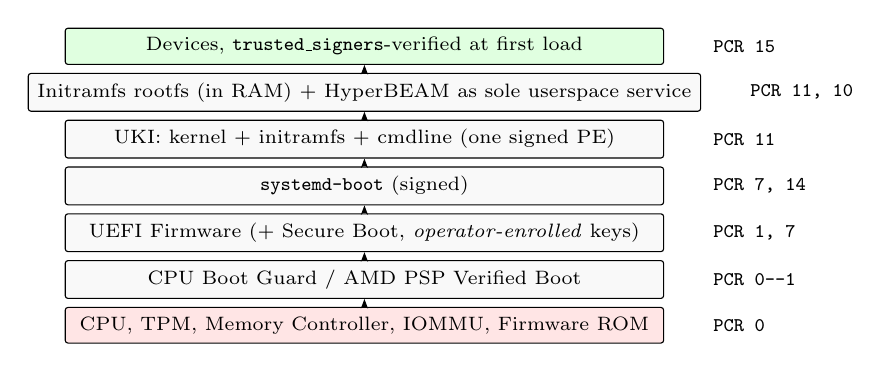
\begin{tikzpicture}[
  node distance=1mm and 5mm,
  every node/.style={font=\scriptsize},
  layer/.style={draw, rounded corners=1pt, minimum height=3.8mm,
                minimum width=76mm, align=center, fill=gray!5},
  pcr/.style={font=\scriptsize\ttfamily, anchor=west},
  arr/.style={-{Stealth[length=1.2mm]}, thick}
]
  \node[layer, fill=red!10]        (hw)   {CPU, TPM, Memory Controller, IOMMU, Firmware ROM};
  \node[layer, above=of hw]        (bg)   {CPU Boot Guard / AMD PSP Verified Boot};
  \node[layer, above=of bg]        (uefi) {UEFI Firmware ($+$ Secure Boot, \emph{operator-enrolled} keys)};
  \node[layer, above=of uefi]      (sb)   {\texttt{systemd-boot} (signed)};
  \node[layer, above=of sb]        (uki)  {UKI: kernel $+$ initramfs $+$ cmdline (one signed PE)};
  \node[layer, above=of uki]       (fs)   {Initramfs rootfs (in RAM) $+$ HyperBEAM as sole userspace service};
  \node[layer, above=of fs, fill=green!12] (dev) {Devices, \texttt{trusted\_signers}-verified at first load};
  \node[pcr, right=of hw.east]   {PCR 0};
  \node[pcr, right=of bg.east]   {PCR 0--1};
  \node[pcr, right=of uefi.east] {PCR 1, 7};
  \node[pcr, right=of sb.east]   {PCR 7, 14};
  \node[pcr, right=of uki.east]  {PCR 11};
  \node[pcr, right=of fs.east]   {PCR 11, 10};
  \node[pcr, right=of dev.east]  {PCR 15};
  \draw[arr] (hw)--(bg); \draw[arr] (bg)--(uefi); \draw[arr] (uefi)--(sb);
  \draw[arr] (sb)--(uki); \draw[arr] (uki)--(fs); \draw[arr] (fs)--(dev);
\end{tikzpicture}
\vspace{-0.3em}
\caption{Trust chain. Every layer from firmware through HyperBEAM binary is
in the TPM signature base by direct measurement: the kernel, initramfs and
cmdline together compose a single PE atomically hashed into PCR 11, so
every byte of HyperBEAM and the Erlang runtime is covered.}
\label{fig:stack}
\vspace{-0.5em}
\end{figure}

\paragraph{Boot and workload measurement.} CPU-fused Boot Guard / PSP
Verified Boot anchors firmware integrity. UEFI Secure Boot with operator-
enrolled PK/KEK/db ensures only HyperBEAM-OS-signed code boots (PCR 7).
\texttt{systemd-boot} loads a Unified Kernel Image~\cite{systemd-pcrlock}
--- one signed PE containing kernel, initramfs, and cmdline, atomically
measured into PCR 11 --- whose cmdline carries the dm-verity root
hash~\cite{dm-verity} and IOMMU arguments. Linux runs with
\texttt{lockdown=confidentiality}~\cite{lockdown}, module signature
enforcement, IOMMU strict mode, and \texttt{init\_on\_alloc}/
\texttt{init\_on\_free}. Early init verifies memory-encryption capability
from \texttt{/proc/cpuinfo} (\texttt{tme} for Intel, \texttt{sme} for
AMD) and refuses to proceed if the CPU has no such capability at all;
the live activation state is reported in the attestation envelope's
\texttt{tme-enabled} signal (derived from the same \texttt{cpuinfo}
flags --- see the vendor programming references~\cite{intel-tme,amd-sme}
for exact semantics) so the verifier's policy engine, not the appliance,
decides whether to accept activation=false.
HyperBEAM is the sole userspace service: its binary (with the Erlang
runtime) lives in the UKI's initramfs, so the kernel, initramfs, cmdline
and HyperBEAM binary together hash into a single atomically-measured PE
covering every byte at PCR 11. The node signs results with RSASSA-PSS,
which produces fresh bytes on each signing of the same message --- relevant
if a consumer treats signature distinctness as an event-freshness signal.
Devices loaded at first use are signature-checked against
\texttt{trusted\_signers}, then assimilated into the Erlang environment;
each first load extends PCR 15 with a named event. The running workload's
\emph{static identity} is thus hardware-rooted, not self-reported; runtime
state is protected by A1 plus memory encryption (\S\ref{sec:memenc}).

\paragraph{Operator key authority.} A defining property of LapEE
relative to cloud TEEs: the operator owns the Secure Boot keys
(PK/KEK/db) for their own appliance, enrolled into UEFI NVRAM via
\texttt{sbctl} at provisioning. Cloud TDX/SEV-SNP deployments instead
grant key authority to the cloud vendor, who chooses which images run
and what their measurements should be. LapEE splits the trust anchor
between two independent parties: the operator decides which images
their machine accepts, and any verifier evaluates against an open trust
anchor (the TPM vendor root) that is not under the operator's control.
Neither party can substitute for the other; the consumer needs both to
agree before accepting a transcript.

\paragraph{Ephemeral node key binding.} At the end of measured boot,
HyperBEAM calls \texttt{TPM2\_Create} for a fresh signing keypair under
a primary on the Endorsement hierarchy. The private key never leaves
the TPM and is discarded on reboot. As the \emph{last step before
attestation}, HyperBEAM extends PCR 15 with three named events: the AK
public-key digest (binds the key to this boot), the running node-
configuration id (binds the workload), and a commitment to the firmware
TCG event log (seeds the AO-Core hashpath, \S\ref{sec:aocore}). A
verifier replaying the event log observes all three land in PCR 15
after all TCB measurements, at which point PCR state is immutable for
the boot's lifetime. Device identity is anchored at the TPM vendor root
via the EK certificate (A2), so an attacker cannot synthesize a fresh
``device'' without vendor collusion. All TPM sessions touching
sensitive state use HMAC $+$ AES-128-CFB parameter
encryption~\cite{tcg-tpm2}.

\paragraph{Attestation evidence.} (i) \texttt{TPM2\_Quote} with verifier-
supplied nonce, AK-signed; (ii) EK certificate read from TPM NV at the
TCG-standard handle, chained to the TPM vendor root; (iii) TCG event
log~\cite{tcg-pcclient}; (iv) HyperBEAM runtime event log (device first-
loads + the three PCR-15 extends above); (v) machine-identifying fields
(CPU, TPM, TME/SME, Secure Boot, IOMMU); (vi) the running node's
configuration message, embedded inline so the verifier can recompute its
identity hash. Every field is a named event-log entry.

\vspace{-0.3em}
\section{AO-Core Continuity: from silicon to signed result}
\label{sec:aocore}
\vspace{-0.3em}

AO-Core~\cite{ao-core} is HyperBEAM's computation model: every message
routes through a pipeline of composable devices; every execution step
extends a cryptographic hashpath over its inputs and outputs. The hashpath
is the same primitive as a TPM event log --- a merkle chain of named,
hashed events --- applied at a different layer of the stack. HyperBEAM
seeds its AO-Core chain with a commitment to the TPM event log tip
immediately after \texttt{key-pubkey-extend}; thereafter every device
first-load and every message extends the chain. The two logs are not
analogous mechanisms; they are the same cryptographic primitive composed
end-to-end (Figure~\ref{fig:chain}).

\begin{figure}[!ht]
\centering
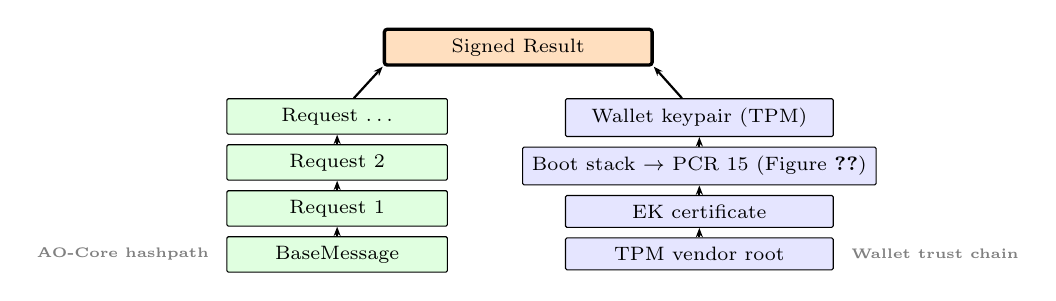
\begin{tikzpicture}[
  node distance=1.2mm and 14mm,
  every node/.style={font=\scriptsize, align=center},
  apex/.style={draw, rectangle, rounded corners=1pt, very thick,
               fill=orange!25, minimum width=34mm, minimum height=4.5mm},
  hp/.style={draw, rectangle, rounded corners=0.5pt,
             fill=green!12, minimum width=28mm, minimum height=3.6mm},
  rot/.style={draw, rectangle, rounded corners=0.5pt,
              fill=blue!10, minimum width=34mm, minimum height=3.6mm},
  arr/.style={-{Stealth[length=1.2mm]}, thick},
  axis/.style={font=\tiny\bfseries, gray}
]
  \node[apex] (top) {Signed Result};

  \node[hp, below=4mm of top.south, xshift=-23mm]  (rN)  {Request $\ldots$};
  \node[hp, below=of rN]                            (r2) {Request 2};
  \node[hp, below=of r2]                            (r1) {Request 1};
  \node[hp, below=of r1]                            (bm) {BaseMessage};

  \node[rot, below=4mm of top.south, xshift=23mm]  (key)  {Wallet keypair (TPM)};
  \node[rot, below=of key]                          (boot) {Boot stack
        $\rightarrow$ PCR 15 (Figure~\ref{fig:stack})};
  \node[rot, below=of boot]                         (ek)   {EK certificate};
  \node[rot, below=of ek]                           (root) {TPM vendor root};

  \draw[arr] (rN)--(top.south west);
  \draw[arr] (r2)--(rN);
  \draw[arr] (r1)--(r2);
  \draw[arr] (bm)--(r1);

  \draw[arr] (key)--(top.south east);
  \draw[arr] (boot)--(key);
  \draw[arr] (ek)--(boot);
  \draw[arr] (root)--(ek);

  \node[axis, left=1mm of bm]    {AO-Core hashpath};
  \node[axis, right=1mm of root] {Wallet trust chain};
\end{tikzpicture}
\vspace{-0.3em}
\caption{The signed result is the apex of two converging chains. Left:
the AO-Core hashpath over the computation --- each request extends a
merkle commitment over the previous step's inputs and outputs, ending
at the result. Right: the constituents that back the signing wallet
--- TPM vendor root anchors the EK certificate, which identifies the
TPM; the operator-signed boot stack (Figure~\ref{fig:stack}) is hashed
into PCR state; PCR 15 binds the ephemeral wallet keypair to that
exact boot. The result's bytes \emph{are} the hashpath tip, signed by
the wallet --- and the wallet exists only because every layer beneath
it verified at boot.}
\label{fig:chain}
\vspace{-0.5em}
\end{figure}

The result of every computation in the system is signed alongside the
hashpath describing how it was made. When the signature is produced by a
LapEE-bound key and the signed artifact is published to
Arweave~\cite{arweave}, a recipient has all the evidence needed to evaluate
trust: CPU architecture, motherboard, firmware version, microcode level,
TPM manufacturer, and memory-encryption state, through the bootloader,
kernel, initramfs, cmdline, rootfs, and HyperBEAM binary measurements,
through the operator's \texttt{trusted\_signers} set, through the
initiation of the computation and every input, and finally to the result.
The ``LapEE'' label in a higher-layer predicate (e.g.,
\texttt{green-zone@1.0}'s \texttt{is-admissible}) is not a vague tier
marker but the conjunction of every concretely-verifiable property in the
attestation. The chain binds the transcript to the boot conditional on A1
--- the same conditional under which TDX or SEV-SNP guest attestations
bind their guest transcripts.

\paragraph{Worked example.} A live boot of the implementation
(\S\ref{sec:implementation}) on a Framework 13 produces an envelope
whose three named PCR-15 extensions land in the order
\texttt{node-identity-extend}, \texttt{key-pubkey-extend},
\texttt{tcg-log-tip-commitment}. The quoted PCR 15 is the iterated
SHA-256 fold of those three digests, starting from the TPM-reset
all-zero state:
\begin{quote}\footnotesize\ttfamily
seq 0  digest = sha256(node-message)\\
seq 1  digest = sha256(ak-pub-pem)\\
seq 2  digest = sha256(tcg-event-log)\\
PCR15  = fold(0..0, [seq0, seq1, seq2])
\end{quote}
A verifier replays the fold from the envelope's runtime event log and
matches it against the quoted PCR 15 byte-for-byte. The seed of the
AO-Core hashpath is the same SHA-256 as the seq-2 digest, so the
hashpath inherits the exact firmware measurement chain rather than
running parallel to it. Two independent reproducible computations land
on the same value: the consumer trusts neither node nor verifier
implementation, only the underlying primitives.

\paragraph{Composition across operators.} A computation that traverses
$k$ LapEE operators yields a chain of $k$ attestations, one per step,
each binding the per-step transcript to a different ephemeral wallet
on a different machine. The hashpath at step $i$ commits to the
hashpath at step $i\!-\!1$, so a step's attestation transitively
covers every prior step's inputs --- but each step's TPM-signed
quote covers only \emph{that step's} measured boot. A consumer
verifies the chain by walking the $k$ attestations in order, checking
each operator's EK chain, each AK's PCR-15 binding to its boot, and
the AO-Core continuity between consecutive steps. Operators are
adversarial by default and need not trust one another; attesting
honestly is in their incentive interest because the network excludes
work that does not chain. Multi-tenant isolation \emph{between
machines} is exactly the property the network supplies in place of
multi-tenant isolation \emph{within} a machine.

\vspace{-0.3em}
\section{Security Argument}
\label{sec:security}
\vspace{-0.3em}

\begin{table}[ht]
\centering
\footnotesize
\begin{tabular}{@{}p{0.32\linewidth} p{0.22\linewidth} p{0.39\linewidth}@{}}
\toprule
\textbf{Attack} & \textbf{Outcome} & \textbf{Mechanism} \\
\midrule
Modified kernel                  & Blocked at load   & UKI signature invalid; Secure Boot refuses. \\
Modified initramfs / cmdline     & Detected in attest.& UKI hash recomputes; PCR 11 diverges. \\
Different signed OS image        & Detected in attest.& PCR 11 diverges; quote binds key to wrong boot. \\
Unsigned kernel module           & Blocked at load   & \texttt{module.sig\_enforce=1}, lockdown. \\
\texttt{/dev/mem}, \texttt{/dev/kmem} & Blocked at load & Absent under lockdown-confidentiality. \\
\texttt{kexec} to attacker kernel & Blocked at load  & Disabled by lockdown. \\
Debugger attach to HyperBEAM     & Blocked at load   & Yama \texttt{ptrace\_scope=3}; lockdown bans \texttt{ptrace(PTRACE\_ATTACH)}, \texttt{/proc/*/mem}. \\
Malicious or modified device     & Blocked at load   & Signature fails against \texttt{trusted\_signers}. \\
Peripheral DMA (PCIe, TB, USB4)  & Blocked at load   & IOMMU strict denies DMA to non-assigned pages. \\
Cold boot of RAM                 & At-rest            & TME/SME key cleared on power loss; residue is ciphertext. \\
DIMM swap, passive bus sniff     & At-rest            & DIMM I/O is AES-XTS ciphertext. \\
Bus replay at same address       & \textbf{Partial} (\S\ref{sec:memenc}) & BEAM immutability, allocator randomization, TPM counters. \\
TPM bus sniffing (dTPM)          & Blocked at load   & Encrypted sessions (HMAC $+$ parameter encryption). \\
Firmware debug (DCI, JTAG)       & Detected in attest.& Debug bits in PCR 0/1. \\
BIOS downgrade                   & Detected in attest.& PCR 0 diverges; verifier version floor. \\
Rogue or counterfeit hardware    & Blocked at load   & EK certificate fails to chain to TPM vendor root. \\
\bottomrule
\end{tabular}
\vspace{-0.3em}
\caption{Attack classes by defense type. Detectable-only attacks succeed
locally but exclude the node from work through any verifier enforcing the
corresponding policy.}
\label{tab:attacks}
\vspace{-0.5em}
\end{table}

\paragraph{Verifier policy as a configuration, not a binary.} Every
\emph{detected-in-attestation} row above resolves at the verifier, not
the appliance. A verifier policy is a small open data structure: an
allow-list of expected PCR values per layer, a minimum OS version
floor, an EK-chain trust set, a set of warn-vs-critical labels, and a
score weighting. The reference implementation's
\texttt{\~{}tpm-interpret@1.0} device renders this as an
\texttt{attested-with-warnings (score)} verdict, with named warnings
the consumer can policy-filter; the same envelope can yield
\emph{accepted} under a permissive policy and \emph{rejected} under a
strict one without re-attestation. Importantly, verifier policy is
public and consumer-chosen, not appliance-chosen --- the appliance
just produces honest evidence.

\subsection{Memory encryption, integrity, and replay}
\label{sec:memenc}
\vspace{-0.2em}

TME and TSME encrypt all DRAM under a per-boot ephemeral AES-XTS key held
in the CPU package. The XTS tweak is the physical address, so ciphertext
cannot be relocated between addresses. A passive attacker reaching DRAM
(cold boot, DIMM swap, bus interposer) recovers ciphertext only.

Plain TME/SME does not provide per-line \emph{integrity} or
\emph{anti-replay} in the fine-grained sense of SGX's Memory Encryption
Engine~\cite{costan-sgx}. SEV-SNP adds Reverse-Map-Table integrity but has
had ciphertext-channel attacks~\cite{cipherleaks}; TDX adds MAC-protected
memory; all still require an honest guest kernel for workload integrity.
LapEE addresses the replay gap with three layers.

\textbf{(1) BEAM immutability.} User-space BEAM state is overwhelmingly
immutable: once a term occupies an address, that address is not
rewritten in its lifetime, so replay at an unchanged address is a no-op.
The residual case is address reuse after GC --- a stale ciphertext
written back into a recycled slot would have to be structurally valid
in its new semantic context, typically false because BEAM tag bits and
internal invariants do not match arbitrary stale bytes (mismatch surfaces
as memory corruption, not a usable term). Probabilistic.

\textbf{(2) Allocator randomization.} Randomize placement within
allocator carriers to further suppress address-reuse. Probabilistic.

\textbf{(3) TPM-backed counters for load-bearing invariants.} Where
anti-replay must be cryptographic, \texttt{\~{}tpm@2.0a} exposes
volatile PCR extend (within-session freshness) and NV counter with
PolicyPCR (monotonic across reboots, tens of ms per increment,
incrementable
only when the golden PCR set is satisfied; for durable single-assignment
invariants such as AO-Core slot heights).

(1)$+$(2) cover BEAM user-space terms only; kernel data, page tables,
DMA rings, allocator metadata, and native buffers fall to the broader
active-DRAM-write concern. The signing key itself lives in the TPM, not
DRAM. Plaintext inputs to sign operations do pass through DRAM, but
tampering with them corrupts the AO-Core hashpath tip and surfaces as
inconsistency to the computation's recipient. The most a user-space
replay can achieve is re-signing an already-signed input; RSASSA-PSS
produces fresh bytes each time, compromising no downstream property
we have identified. Active-write adversaries on DDR4/DDR5 require
lab-grade bus interposers in the same cost class as the chip-decap
attacks all deployed TEEs accept as out of scope.

\vspace{-0.3em}
\section{Residual Threats}
\vspace{-0.3em}

\emph{Physical attack on the CPU or TPM package} (decap, fault injection,
laser, FIB) is accepted as a hardware-attack-complexity bar, consistent
with TDX, SEV-SNP, and Apple PCC. \emph{Kernel 0-days} (A1) are mitigated
by signed image updates, a verifier-enforced OS version floor, and minimal
userspace. \emph{Compromise of a trusted signing party} is bounded by
multi-party signing, reproducible builds, and public rotation logs.
\emph{TME/SME key side channels} have no published full break to date; the
primitive is simpler than SGX's MEE and accordingly less studied.
\emph{Liveness} and \emph{traffic analysis} are out of scope, addressable
at the network layer by redundancy and padding/mixing respectively.

\vspace{-0.3em}
\section{Hardware Availability}
\label{sec:availability}
\vspace{-0.3em}

\begin{table}[ht]
\centering
\footnotesize
\begin{tabular}{@{}p{0.33\linewidth} p{0.33\linewidth} p{0.24\linewidth}@{}}
\toprule
\textbf{Class} & \textbf{Silicon capability} & \textbf{BIOS exposure} \\
\midrule
Intel vPro (client, 11th gen+)    & TME since Tiger Lake 2020   & $\sim$70--80\% \\
Intel non-vPro (client, 11th gen+)& TME capable, patchy         & $\sim$20--30\% \\
Intel Xeon SP                     & TME since Ice Lake-SP 2021  & $\sim$95\% \\
AMD Ryzen Pro                     & TSME since Zen 2 2019       & $\sim$70--80\% \\
AMD Ryzen consumer                & TSME capable, patchy        & $\sim$20--40\% \\
AMD EPYC                          & SME/TSME since Naples 2017  & $\sim$95\% \\
\midrule
TPM 2.0                           & Win 11 requirement 2021     & $\sim$100\% \\
IOMMU                             & Business-class $\geq$ 2012  & $\sim$100\% bc \\
UEFI Secure Boot (enrollable PK)  & Win 8 era 2012              & $\sim$95\% \\
\bottomrule
\end{tabular}
\vspace{-0.3em}
\caption{Primitive availability; engineering estimates from vendor feature
tables, Windows 11 requirements, and community compatibility lists.}
\label{tab:hw}
\vspace{-0.5em}
\end{table}

Per-feature composition (product of rates) yields $\sim$11--35\% viability
on random consumer laptop purchases, rising above $\sim$70\% filtered to
business-class secondary market (ThinkPad T/X/P, Latitude, EliteBook) where
per-feature rates cluster above 90\%. Contrast: TDX-capable silicon
(Sapphire Rapids$+$) is low-single-digit percent of the x86 server
installed base (industry estimates); SEV-SNP similar; client CVM TEEs do
not meaningfully exist. LapEE thus addresses an installed base roughly an
order of magnitude larger at one to two orders of magnitude lower per-
machine cost, often including zero-cost hardware already in operator
possession.

\vspace{-0.3em}
\section{Implementation and demonstration}
\label{sec:implementation}
\vspace{-0.3em}

\paragraph{Implementation.} The architecture ships in the LapEE
repository root. A
from-scratch Buildroot kernel ($\sim$12 MB \texttt{bzImage}) with the
hardened symbol set described in \S\ref{sec:architecture}, the
HyperBEAM release with the \texttt{lapee\_tpm} NIF over libtss2, the
LapEE init script, and Intel/MediaTek WiFi userspace are packed into
one signed UKI ($\sim$73 MB) on a UEFI-bootable USB image. The
\texttt{\~{}tpm@2.0a} device wraps tpm2-tss~\cite{tpm2-tss} for
quote, sign, PCR-extend, NV ops, and event-log-read, with HMAC +
AES-128-CFB parameter-encrypted sessions on every TPM operation that
touches sensitive state. Operator bring-up is three commands: enroll
PK/KEK/db; \texttt{make runtime-write}; boot the
target. The boot splash decides its own phase machine
(\texttt{boot}~$\rightarrow$~\texttt{net-up}~$\rightarrow$~\texttt{hb-wait}~$\rightarrow$~\texttt{ready}),
prints the URL when HyperBEAM answers \texttt{/info}, and stays
running as PID 2.

\paragraph{Demonstrated boot.} A Framework 13 (13th Gen Intel Core,
Nuvoton dTPM, INSYDE H2O 03.04) boots from a 1 GB USB stick to
attestation-serving in roughly 25 seconds on a cold cache. The
envelope returned at \texttt{/\~{}tpm@2.0a/attestation} is 105 KB
and contains the EK certificate read from TPM NV at handle
\texttt{0x01C00002} (1.2 KB; chain-validated against the Nuvoton
ECC521 root via the ECC384 Leaf CA), the AK public PEM
(endorsement-hierarchy primary, RSA 2048), a \texttt{TPM2\_Quote}
over PCRs $\{0,1,7,10,11,14,15\}$, the firmware TCG event log (3.1
KB, kernel-sourced via \texttt{securityfs}), the HyperBEAM runtime
event log (the three PCR-15 extensions), the running node
configuration with its \texttt{hb\_message:id} hash, and inline
platform probes from DMI, \texttt{/proc/cpuinfo}, and the kernel's
lockdown / Secure-Boot variables. The signing wallet is the AK;
results signed by it carry the full trust chain of
Figure~\ref{fig:chain} as a single transcript.

\paragraph{Verifier output.} An external Python verifier (separate
codebase, separate language, no shared state with the producer) runs
offline against the envelope and reports six checks:
\begin{quote}\footnotesize\ttfamily
[PASS] EK cert chains to NUVOTON ECC521 RootCA via ECC384 LeafCA\\
{}[PASS] TPM2\_Quote signature + pcrDigest + nonce all valid\\
{}[PASS] Runtime event log replay of PCR 15 matches quoted value\\
{}[PASS] PCR 15 seq=0 commits to node-message-id\\
{}[PASS] PCR 15 seq=1 commits to AK pub PEM\\
{}[PASS] Embedded node-message + id present and 32-byte b64url\\
VERDICT: ATTESTATION ACCEPTED
\end{quote}
The in-tree \texttt{\~{}tpm-interpret@1.0} device runs the same checks
plus a wider tier-graded policy and produces an
\emph{attested-with-warnings} dashboard verdict at score 92/100; the
sole warning is \texttt{tpm-safe=false} (cross-boot counter-
monotonicity weak under the appliance power-cycle model), which
default LapEE policy accepts because every attestation is already
nonce-fresh per \S\ref{sec:architecture}. Strict policies that
mandate counter-monotonicity may reject; verdict surface is the
operator/consumer's policy lever, not the appliance's.

\paragraph{Related work.} Apple PCC~\cite{apple-pcc} is architectural
precedent but assumes Apple-owned hardware and facility.
Naik~\cite{naik-dginf} attempts similar on Apple Silicon; defeated by
the absence of a third-party-accessible measurement register.
Keylime~\cite{keylime} implements verifier-side policy;
RATS~\cite{rfc9334} standardises terminology;
BuilderNet~\cite{flashbots-buildernet} uses TDX-attested decentralized
compute, but in the dominant TDX deployment the operator supplies both
image and expected measurement --- circular trust LapEE avoids via
operator-enrolled Secure Boot and reproducible source.

\paragraph{Conclusion.} For the decentralized-compute threat model a
classical hardware TEE is not required. An attested dedicated appliance
built on commodity primitives trades only single-machine multi-tenant
isolation --- which the network does not need, because it provides
tenancy by distributing work. LapEE is a primitive; higher-layer
predicates compose on top. The ingredients ship in ordinary business
hardware today.

\vspace{0.4em}
\noindent\footnotesize\textbf{Availability.} Build recipes and the
\texttt{\~{}tpm@2.0a} device ship in the LapEE repository root;
the second verifier sits next to them under
\texttt{secondary-external-verifier/}.

\printbibliography

\end{document}
